\documentclass{article}

\usepackage[english]{babel}
\usepackage{hyperref}
\usepackage{graphicx}
%\usepackage{accsupp}
\usepackage{fancyhdr}
\pagestyle{fancy}
%\usepackage{xcolor}
%\usepackage{xparse}
%\usepackage{tabularx}
\usepackage{longtable}
\usepackage{array}
\usepackage{caption}
\fancyhf{}
\captionsetup{justification=raggedright,singlelinecheck=false}

% Text to make one more indention level:


\usepackage{titlesec}

\titleclass{\subsubsubsection}{straight}[\subsection]

\newcounter{subsubsubsection}[subsubsection]
\renewcommand\thesubsubsubsection{\thesubsubsection.\arabic{subsubsubsection}}
\renewcommand\theparagraph{\thesubsubsubsection.\arabic{paragraph}} % optional; useful if paragraphs are to be numbered

\titleformat{\subsubsubsection}
  {\normalfont\normalsize\bfseries}{\thesubsubsubsection}{1em}{}
\titlespacing*{\subsubsubsection}
{0pt}{3.25ex plus 1ex minus .2ex}{1.5ex plus .2ex}

\makeatletter
\renewcommand\paragraph{\@startsection{paragraph}{5}{\z@}%
  {3.25ex \@plus1ex \@minus.2ex}%
  {-1em}%
  {\normalfont\normalsize\bfseries}}
\renewcommand\subparagraph{\@startsection{subparagraph}{6}{\parindent}%
  {3.25ex \@plus1ex \@minus .2ex}%
  {-1em}%
  {\normalfont\normalsize\bfseries}}
\def\toclevel@subsubsubsection{4}
\def\toclevel@paragraph{5}
\def\toclevel@paragraph{6}
\def\l@subsubsubsection{\@dottedtocline{4}{7em}{4em}}
\def\l@paragraph{\@dottedtocline{5}{10em}{5em}}
\def\l@subparagraph{\@dottedtocline{6}{14em}{6em}}
\makeatother

\setcounter{secnumdepth}{4}
\setcounter{tocdepth}{3}

\makeatletter
\newcommand{\definestring}[2]{\@ifdefinable{#1}{\gdef#1{#2}}}
\makeatother

% end.


\chead{
\includegraphics[width=1cm]{images/icon-black.pdf}}
\cfoot{\thepage}

\author{phseiff\\ \href{https://phseiff.com}{from phseiff.com}}

\title{\begin{center}
           %\BeginAccSupp{method=plain,Alt={\{gender*render\}\\Specification}}
           
\includegraphics{images/title-black.pdf}
           %\EndAccSupp{}
\end{center} Template system and implementation specification for rendering gender-neutral email templates with pronoun information}

\begin{document}
\maketitle
\tableofcontents

\section{Abstract}

    Our society, as well as the way we perceive gender, are steadily evolving.
    This evolution does not hold in light of technological questions, and it is our -the "IT people"'s duty- to address and do our best to solve the social issues that arise from our technology.
    One such technology are email- and other text templates, which are becoming increasingly popular to automate customer interactions of any kind, be it in newsletters, notifications or program menus.
    Many such templates are gender-specific, in that they address the reader in a gendered fashion ("Dear Mrs. Dursley, ...").
    Such templates are relatively easily implemented by providing two versions of the email, one for every binary gender.
    However, some texts are far more complicated, because they address multiple people (each with their own unknown at the time of writing), or people in the third person (throwing their pronouns into the mix).
    In addition, an increasingly height amount of people use non-binary pronouns, or gender-neutral pronouns, many of whom might now yet be discovered at the time of writing, which makes these people marginalized when it comes to being correctly addressed even in automated emails.\\

    This creates the requirement for creating template systems for the english language, and, in extention, any language (since all languages work differently), that support writing complex texts in a gender-neutral fashion and later "render" them to correctly gendered texts.\\

    \{gender*render\} is an attempt at creating one such template language, including a Specification, to serve as a proof of concept as well as a starting point for people who want to implement similar things.
    The vision behind this proof of concept is not only to show \emph{how} addressing people with unconventional preferred pronouns can be automized, but also to show \emph{that} it can be easily automized, to debunk the myth that properly addressing non-binary people in an automated fashion is simply technically impossible.

\section{Requirements}

    There are multiple requirements for such a template language, whom I will list here, including short explanation of why they are required wherever I deem it necessary:

    \begin{itemize}
        \item The language must be easy to use even for less tech affine people.
              This means that the atoms of the language, such as tags et cetera, must be as short as possible, and should not clash with commonly used words or signs, so the amount of escape characters the user needs to use is minimal.
        \item The language must support different scenarios:
        \begin{itemize}
            \item One person being addressed versus multiple people being addressed
            \item Only people mentioned in first person, only people mentioned in third person, or a mixture of both
            \item Everyone using pronouns versus some people preferring not to use any pronouns
        \end{itemize}
        \item The fact that multiple scenarios are supported may not make using the template language for only a subset of them more complicated that it needs to be.
        \item Rendering templates may only require the information needed for rendering the template.
        For example, rendering a template that never addresses anyone in the first person should not require providing information as to whether the person goes by "Mr", "Mrs" or any other form of address.
        This is especially relevant since users do not want and should not need to require more information that necessary for rendering the templates, especially considering the intimate nature of preferred pronouns.
        \item The syntax should be describable using a context-free grammar in conjunctive normal form, which allows easy syntax checking and syntax highlighting.
        \item The data containing a persons preferred pronouns should be given in a widely-used, standardized format, such as JSON.
    \end{itemize}

\section{Design Decisions}

    The following decisions where made based on the the technical requirements ruled out in the corresponding section:

    \begin{itemize}
        \item The language uses a syntax similar to pythons build-in string formatting syntax, using curly brackets to annotate gender-specific parts of a sentence.
        Backslashes are used as escape characters for the rare occurrences where curly brackets are actually needed.
        \item In addition to terms like "possessive pronoun", using the gender-neutral form ("their") in tags is supported, potentially making texts more fluid to write and easier to read in their un-rendered form.
        \item If tags contain IDs to annotate which person is referred to, a mapping of IDs to pronoun preferences is accepted for rendering.
        If no such IDs are added to the document because only one person of unknown gender is addressed in the document, the pronoun preferences are directly accepted by the renderer, without having to be part of a person-to-pronoun-mapping.
        This supports referring to multiple persons in one text without making the writing of texts that refer to only one person any more troublesome.
        \item The pronoun information is given to the renderer as a piece of JSON data (or a similar object if the language used by the implementation supports such objects, e.g. dicts in Python, but strings of JSON data should always be supported).
        Information that is not required by the template may be left out in the template.
        \item Templates can be parsed before being rendered and then used for multiple renderings.
        This should debunk the idea that gender-sensitive template systems are to inefficient to use them.
    \end{itemize}

    These design decisions contain only those that are relevant to the requirements listet in the previous section;
    in-depth explanation and definition of the way the template system works are given in the next section.

\section{Standard}

    This section contains the actual standard.
    It is divided into three subsections;
    one for defining the template language and how gender-neutral texts are described with it,
    one for defining the data structure used to describe the pronoun preferences of all people mentioned in a template,
    and one for guidelines and specification on implementing a renderer for the template language.\\

    The terms "MUST", "MUST NOT", "SHOULD", "SHOULD NOT" and "MAY" in this document are used as defined by the \href{https://tools.ietf.org/html/rfc2119}{RFC 4627}.
    Additionally, the term *does* implies that it *must do*, not that it *can do*.

    \subsection{Template Language}

    Any text that follows the syntax of the following definition is considered a valid \{gender*render\}-template.
    Any text that does not follow the following is not considered a valid \{gender*render\}-template.
    Files whose content is a valid \{gender*render\}-template are referred to as files containing \{gender*render\}-templates in the following section, and \emph{not} as \{gender*render\}-templates on their own.
    It is recommended to save such files with the file type \texttt{.grt} (short for "gender render template").\\

    The purpose of \{gender*render\}-templates is to write texts in a gender-neutral way (at least in regards to some of the individuals they refer to), and to be valid input for the \{gender*render\}-renderer, who is described in a later section.\\

    \{gender*render\}-templates may contain an arbitrary number (including zero) of \{gender*render\}-tags.
    A \{gender*render\}-tag is defined a sequence of characters that starts with an unescaped left curly bracket ("\texttt{\{}", \texttt{U+007B}) and ends with an unescaped right curly bracket ("\texttt{\}}", \texttt{U+007D}) without containing any unescaped curly brackets (\texttt{U+007B} as well as \texttt{U+007D}) in between.
    The purpose of \{gender*render\}-tags is to describe gender-specific sentence components in a gender-neutral fashion, these usually being mentions of a person in the third person singular.\\

    A character is considered escaped if it is proceeded by an unescaped backslash ("\texttt{\textbackslash}", \texttt{U+005C}) or by a backslash which is not proceeded by other backslash.
    A backslash which is not escaped is called an escape-character.
    A template which contains backslashes which are neither escaped nor escape characters is not considered a valid \{gender*render\}-template, as is any template which contains unescaped curly brackets who are not part of any valid \{gender*render\}-tag.\\

    Every character of a \{gender*render\}-tag except the first and last characters (the brackets) is considered part of its content.
    Said content is divided into sections through unescaped asterisks ("\texttt{*}", \texttt{U+002A}).
    A section of a \{gender*render\}-tag does not contain any unescaped asterisks, and it must contain at least one non-whitespace\footnote{"Whitespace" as defined by the \href{https://infra.spec.whatwg.org/\#ascii-whitespace}{HTML Living Standard}.} character.
    Colons ("\texttt{:}", \texttt{U+003A}) are considered special characters in sections, and may thus appear at most once per section, and neither as the first nor as the last non-whitespace  character of the section.
    If a section contains a colon, the characters of the section beforehand the colon (minus all leading or trailing whitespace) are called the sections \emph{type descriptors}, and the characters following the colon (after having all their whitespace collapsed into one \texttt{U+0020}-space each, except for trailing and leading whitespace, which is removed completely) are called the sections \emph{value}.
    If a section does not contain a colon, its \emph{value} is defined as all of its characters (having all their whitespace collapsed into one \texttt{U+0020}-space each, except for trailing and leading whitespace, which is removed completely).\\

    There are multiple different types of section, assigned to sections by their type descriptor.
    A section whose type is "foo" is called a "foo-section".
    Every type of section has a unique priority, as a real number between 0 and 1000, assigned by this specification.
    The right-most section with no type descriptor and no assigned section type is assigned the section type with the highest priority of all section types that no section of the tag is assigned by this rule or its section descriptor yet.
    Every \{gender*render\}-tag must have at least one section, and may only have one section of every type;
    this takes into account the assigned section type of sections without a type descriptor.
    In addition, a tag may not contain more sections than there are section types defined by the spec.\\

    The most basic type of section is the \texttt{context}-type, which describes the syntactic context of the \{gender*render\}-tag.
    Every \{gender*render\}-tag must have one context-section.
    The following table lists the possible values a \texttt{context}-section's value may have, as well as their meanings, though the syntactic validity of the template does not depend on whether the values and types of the the \{gender*render\}-tags are listed in this spec:

    %\begin{minipage}{\linewidth}
    %\pagebreak[5]
    \begin{flushleft}
        \begin{center}
            \begin{longtable}{| >{\raggedright\arraybackslash}p{7em} | >{\raggedright\arraybackslash}p{9em} | >{\raggedright\arraybackslash}p{14em} |}
                 \hline
                 {syntactic context indicated by the value(s)} & {possible values,\linebreak synonymous to each other} & {short explanation, where\linebreak necessary} \\
                 \hline\hline
                 Subject & they, subject, subj & \\
                 \hline
                 Object & them, object, obj & \\
                 \hline
                 Dependant possessive\linebreak Determiner & their, dposs, dpossessive & \\
                 \hline
                 Independent possessive\linebreak Determiner & theirs, iposs, ipossessive & \\
                 \hline
                 Reflexive & themself, reflexive, reflex & \\
                 \hline
                 \hline
                 Form of Address & Mr, Mrs, Mr\_s, address & \\
                 \hline
                 Surname & Smith, name, surname, family-name & (It should be mentioned that Smith is the most common US surname\footnote{according to \href{https://www.voanews.com/usa/all-about-america/most-popular-last-name-each-us-state}{voanews.com}})\\
                 \hline
                 Personal name & Avery, personal-name, first-name & (It should be mentioned that Avery is the most popular unisex name in the US today\footnote{according to \href{https://nameberry.com/unisex-names}{nameberry.com}})\\
                 \hline
                 \hline
                 Custom property & "\texttt{<}" \emph{property} "\texttt{>}" & \emph{property} can be any string without whitespace, and refers to a property of an individual that is defined by its pronoun data as a string, yet not part of the spec. \\
                 \hline
                 \hline
                 Gender-specific Noun & any nominative, with whitespaces replaced by underscores ("\texttt{\_}", \texttt{U+005F}) & If the value of the \texttt{section} does not match any of the above, its content is understood as being a noun which either server as a substitution or as a description of a person.
                 For example, the sentence "\{name\} is an \{actor\}" or "the \{actor\} asked for applause" would be good candidates for using said type of value since "actor" has two different gendered forms ("actor" and "actress") in english. \\
                 \hline
                \caption{Types of context values in tags}
            \end{longtable}
        \end{center}
    \end{flushleft}
    %\end{minipage}

    The priority the \texttt{context}-section type is \texttt{1000}.
    If the \texttt{context}-section's value contains multiple strings, each separated from each other by whitespace, such as "\texttt{\{foo:bar * context:Mr\_s Smith\}}", the \{gender*render\}-tag is interpreted as if it was "\texttt{\{foo:bar * context:Mr\_s\} \{foo:bar * context:Smith\}}", in the form of two different tags separated by a single space ("\texttt{ }", \texttt{U+0020}) and different only in their context value. \\

    The other section type supported by this version of this Specification is the \texttt{id}-type.
    The value of an \texttt{id}-section may take any value as long as it does not contain any whitespace.
    It describes which individual the \{gender*render\}-tag refers to.
    Two \{gender*render\}-tags with the same id-value refer to the same individual.
    The id-value can be omitted by the user if there is only one individual mentioned in the whole template, and in some other cases;
    this is explored further in the renderer section.
    Whether there is an \texttt{id}-section is not part of the template specification, since it is not clear until the pronoun information is given.\\

    Since there are only two section types defined by this specification, and one of them is mandatory, there is no practical need to use any section descriptors.
    They are still defined as a language feature in this template to provide a way to port the template language to other natural languages that might require additional information without having to introduce new syntax elements for every language.\\

    To end this section of the spec, here is a graphic of the \{gender*render\}-template syntax described as a finite state machine (not taking into account the fact that not every section type is valid, and the rules about assigned sections and every type of section only existing once):\\

    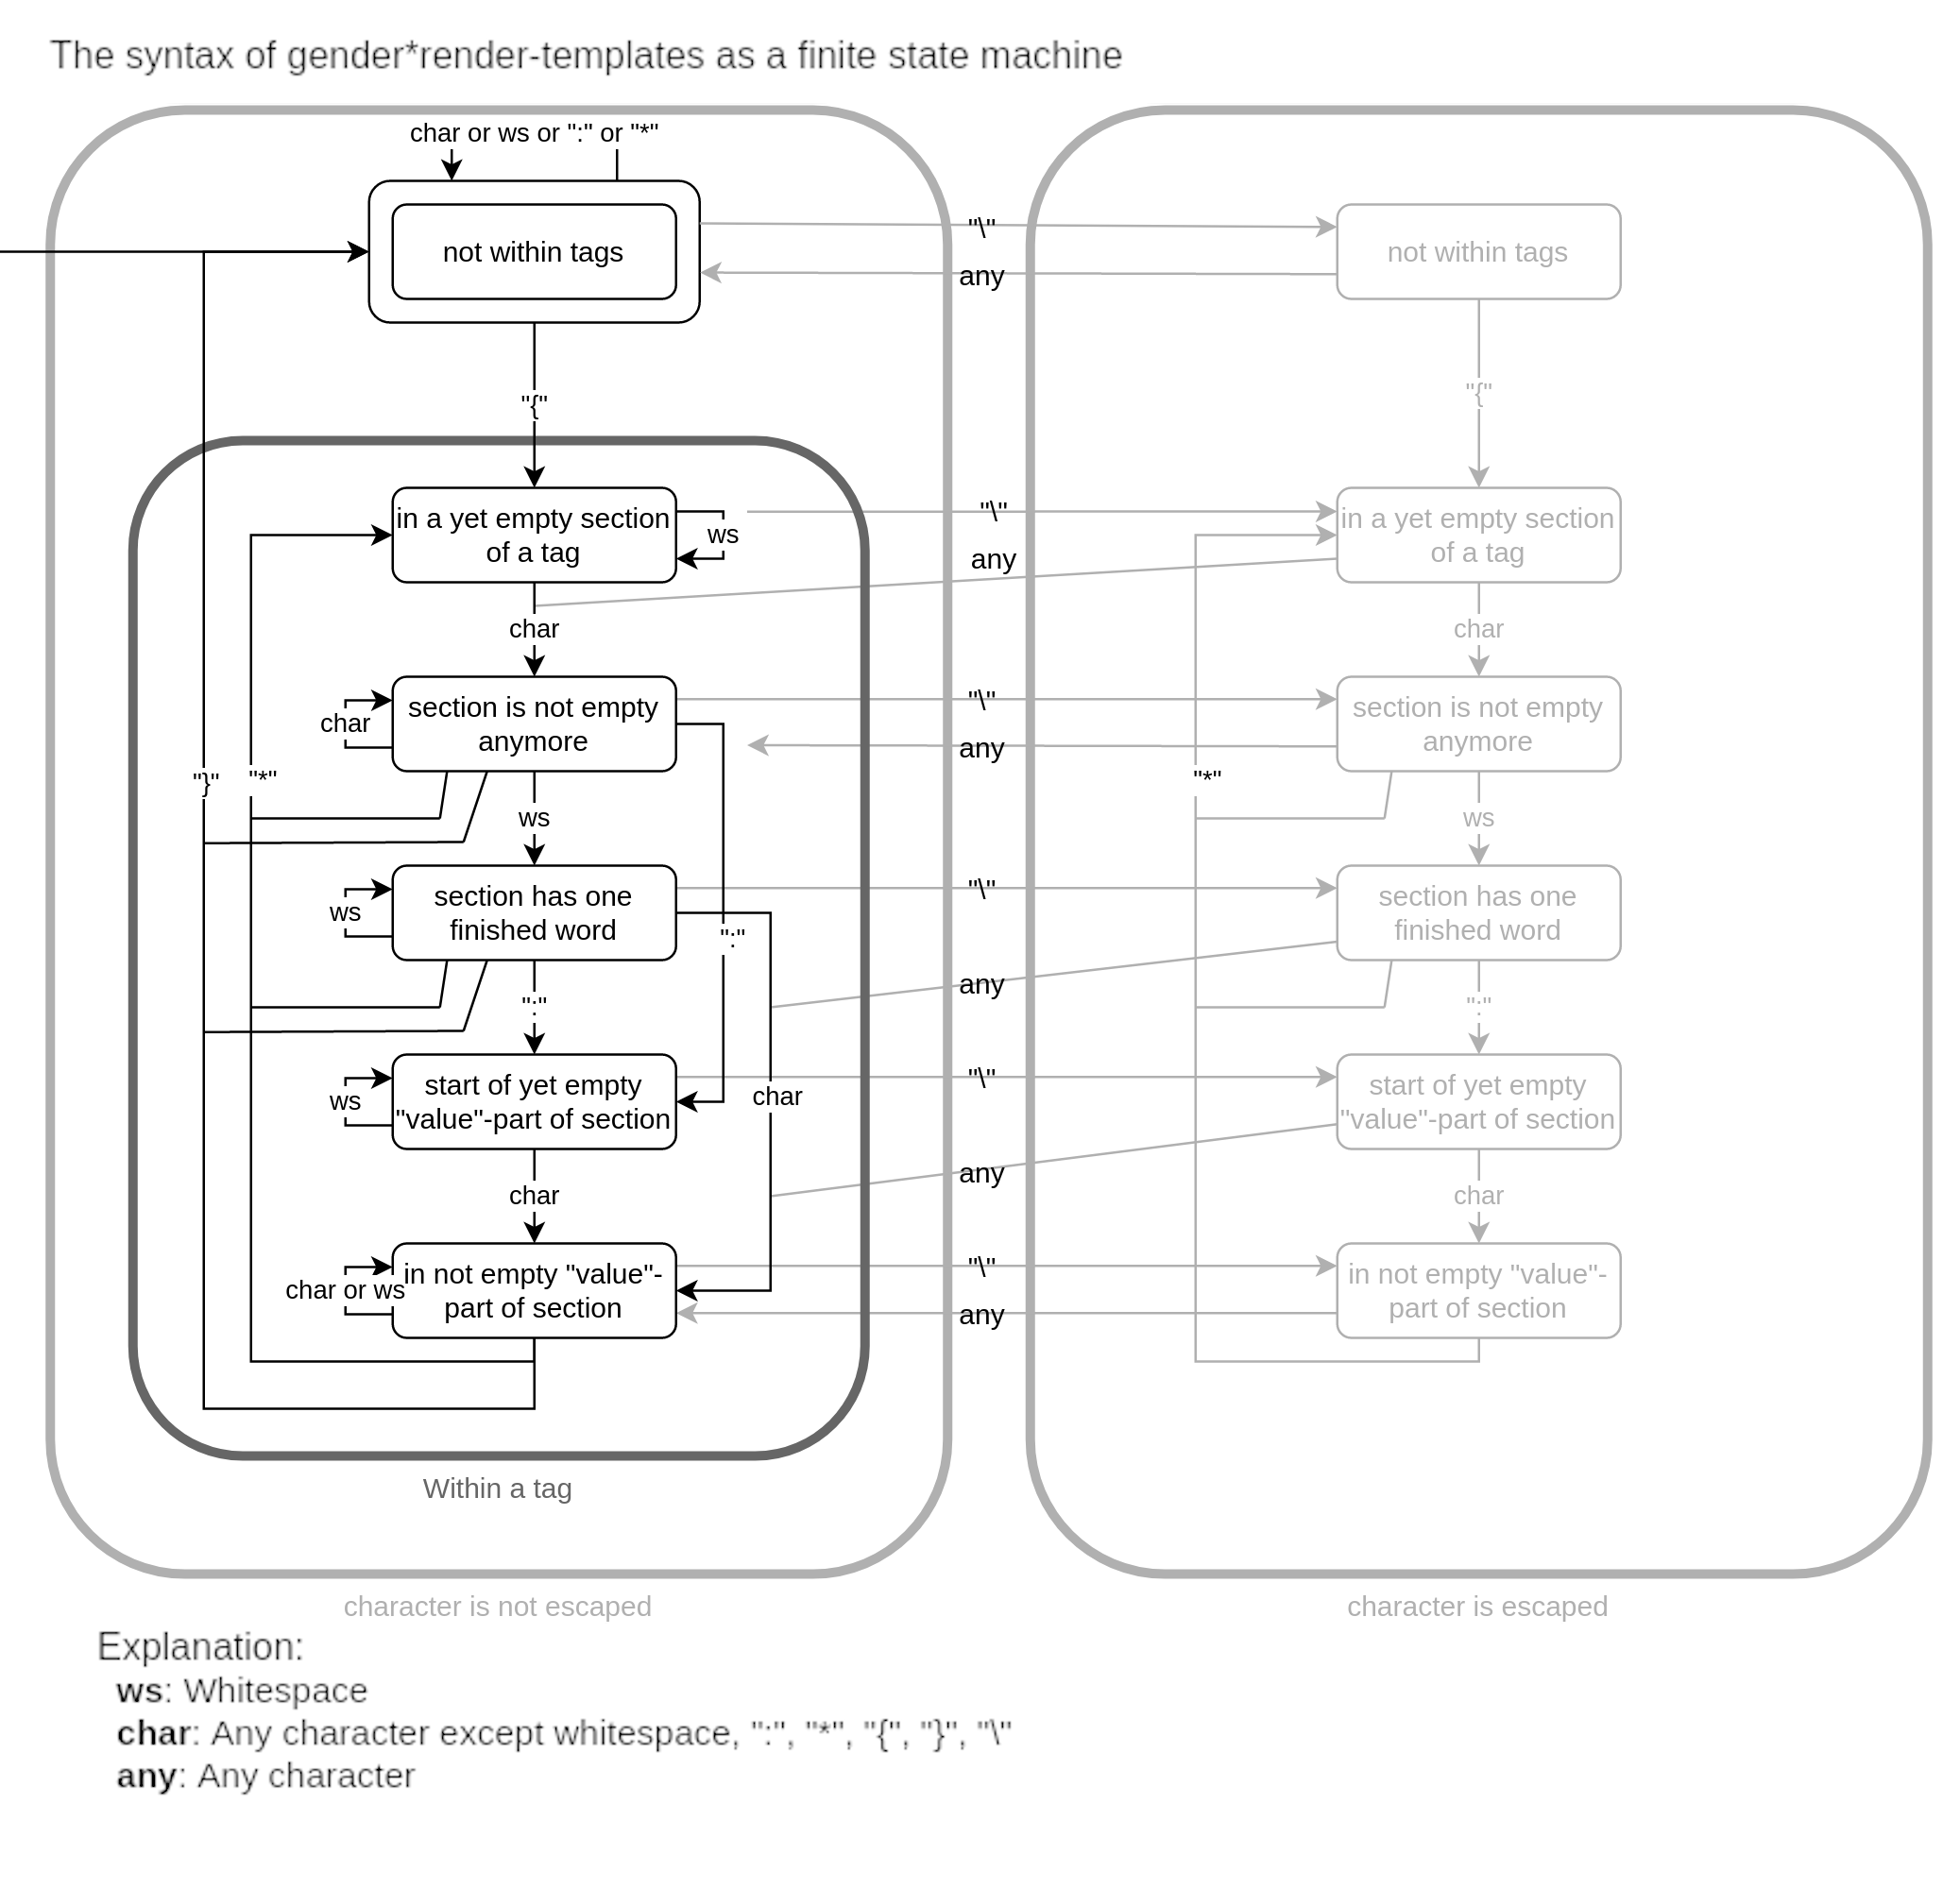
\includegraphics[width=12cm]{images/template-as-finite-state-machine.png}

    \subsection{Pronoun Description Data}

     Pronouns description data, to which we will refer as \{gender*render\}-pronoun-data for the rest of this essay to spare us some words, is the way the user tells the render the pronouns of all people mentioned in a template so the renderer can render it.
     Any piece of text that fits the criteria described below is considered \{gender*render\}-pronoun-data, yet not every such piece of text necessarily works with every template, since it must provide the information required by the template for the rendering to work.
    Files that contain \{gender*render\}-pronoun-data should use the file extension \texttt{.grpd}.\\

    \{gender*render\}-pronoun-data is a type of json data, which makes it easily parsable by any language.\\

    To describe a single individuals pronouns (to which we will refer to as individual pronoun data), a json object is used;
    several of these are then combined to provide pronoun data for all individuals.
    If a piece of individual pronoun data is written into a file, the file extension \texttt{.gripd} should be used.
    Any json object whose properties are strings without whitespace, and whose items are strings, is valid individual pronoun data, though it might not work with every template depending on the information the template requires.\\

    The following table describes the properties a piece of individual pronoun data may use to give you a rough overview of the way individual pronoun data corresponds to the information provided by the \texttt{context}-section of \{gender*render\}-pronoun tags, which will be relevant in the next section (about the way renderers work).
    Every information that can be provided by individual pronoun data (referred to as an "attribute" here) has multiple properties that can be used to refer to it, as long as only one of them is used in the JSON object;
   otherwise, the individual pronoun data is invalid.
    Note that the last line of the table is a catch-it-all and does not refer to one specific attribute in particular:

    %\pagebreak[5]
    \begin{flushleft}
        \begin{center}
            \begin{longtable}{|>{\raggedright\arraybackslash}p{7em} | >{\raggedright\arraybackslash}p{9em} | >{\raggedright\arraybackslash}p{14em} |}
                 \hline
                 information provided by properties (attribute) & property name(s), \linebreak synonymous to each other & short explanation, where necessary\\
                 \hline\hline
                 Subject & they, subject, subj & \\
                 \hline
                 Object & them, object, obj & \\
                 \hline
                 Dependant possessive\linebreak Determiner & their, dposs, dpossessive & \\
                 \hline
                 Independent possessive\linebreak Determiner & theirs, iposs, ipossessive & \\
                 \hline
                 Reflexive & themself, reflexive, reflex & \\
                 \hline
                 \hline
                 Form of Address & Mr, Mrs, Mr\_s, address & \\
                 \hline
                 Surname & Smith, name, surname, family-name & \\
                 \hline
                 Personal name & Avery, personal-name, first-name & \\
                 \hline
                 \hline
                 Gender-specific addressing & gendered-addressing, gendered\_addressing & If set to 0, "False" or "false", the first name of an individual is used instead of its adressation.\\
                 \hline
                 Gender-specific Noun handling & gender-nouns, gender\_nouns & Describes whether the person wants gender-specific nouns to use the female version where possible (e.g.\ "actress" instead of "actor"), the male version where possible (e.g.\ "fireman" instead of "firefighter"), or the gender-neutral version where possible (e.g.\ "firefighter").
                 Possible values for this property are \texttt{"female"}, \texttt{"male"} and \texttt{"neutral"}. \\
                 \hline
                 \hline
                 Custom property & \emph{property\_name} & Corresponds to "\texttt{<}\emph{property\_name}\texttt{>}" in \{gender*render\}-tags. \\
                 \hline
                \caption{Supported properties in individual pronoun data}
            \end{longtable}
        \end{center}
    \end{flushleft}

    \{gender*render\}-pronoun-data is simply a json object whose properties are ids (strings without whitespace) corresponding to ids of \{gender*render\}-tags, and whose items are the individual pronoun data corresponding to their respective ids.
    Since the ids used by the \{gender*render\}-pronoun-data need to correspond to those used by the template, not every valid piece of \{gender*render\}-pronoun-data worked with every template.
    As specified later in the spec, renderers accept \{gender*render\}-pronoun-data as well as individual pronoun data in cases where no or only one id is used.

    \subsection{Pronoun Renderer}

    This section describes the way \{gender*render\}-specification conforming pronoun renderers work.
    It is divided into two subsections, one defining a \{gender*render\}-renderer, and one defining (additional) implementation guidelines that should be followed to ensure that all renderers use similar interfaces and users understand the renderer even if they used to work with a different implementation beforehand.
    The \{gender*render\} implementation that comes with this specification (\url{https://github.com/phseiff/gender-render}) also follows all of these guidelines.

    \subsubsection{Pronoun Renderer specification}

    Any program that follows the specifications below is considered a \{gender*render\}-renderer.
    The purpose of such programs is to take \{gender*render\}-templates and \{gender*render\}-pronoun data and render them to texts that are gendered correctly according to the preferences voiced in the pronoun data.
    We will refer to \{gender*render\}-renderers simply as renderers for the rest of this section to aid the reading flow.\\

    A renderer must take at least two inputs, a \{gender*render\}-template and a piece of pronoun data.
    As for the piece of pronoun data a renderer accepts, every renderer must accept \{gender*render\}-pronoun data as well as individual pronoun data, which is then processed into full \{gender*render\}-pronoun data following a number of steps explained below.
    The renderer may also be written in a way that allows to pass it a path to a \texttt{.gr}-file containing a \{gender*render\}-template instead of the template directly, or even in a way which exclusively allows this way of usage, though the later is not recommended and does not comply with the implementation suggestions given by this document.
    Analogously, the renderer may be written in a way that allows to pass it a path to a \texttt{.grpd}-file containing \{gender*render\}-pronoun data or a path to a \texttt{.gripd}-file containing individual pronoun data instead of the content of the \{gender*render\}-pronoun data directly, or even in a way which exclusively allows this way of usage, though the later is not recommended and does not comply with the implementation suggestions given by this document.\\

    Along the rendering process, several errors might occur for several reasons.
    The way errors are classified and communicated to the user is not an implementation detail, but a part of the specification, since classifying errors is especially important due the logical, yet sometimes contra intuitive way \{gender*render\} renders templates.
    This specification thus defines not only what should raise an error, but also suggests different error names for different types of errors.\\

    If the language of the implementation allows defining and raising custom error types, these error types must be defined and risen accordingly.
    If the language does not allow to define custom error types, yet allows to return information even if the execution of a program or function fails, the program or function must return information indicating what type of error occurred in a reasonable way.
    However, if the language of the implementation provides a standardized way to indicate a function failed to run, yet does not provide a way to return additional information about the cause of this failure, the implementation should use the standardized way of failing if an error occurs instead of returning information about the cause of failure.\\

    The following types of errors are defined by this specification, and are used as described below.
    Please note that whilst the names of the errors are always written in camel case throughout this specification, the way they are written should be according to the official style guide of the language they are implemented in, if there is any.
    If the naming conventions of the language comply with the names of the errors defined in this specification, or if the language does not have any naming conventions, the names defined in this specification must be used.

    \begin{flushleft}
        \begin{center}
            \begin{longtable}{|>{\raggedright\arraybackslash}p{13em} | >{\raggedright\arraybackslash}p{19em} |}
                 \hline
                 Error name & commonly used for \\
                 \hline\hline
                 \texttt{SyntaxError} & Used if the input not a valid template and pronoun data aren't valid, independent of the way they relate to each other. \\
                 \hline
                 \texttt{IdResolutionError} & Used if matching individual pronoun data to tags does not wo out.\\
                 \hline
                 \texttt{MissingInformationError} & Used if the individual pronoun data a tag refers to does not contain the information the tag requires.\\
                 \hline
                 \texttt{DoubledInformationError} & Used if individual pronoun data defines a property multiple times with different names (possible since \{gender*render\} defines multiple different names for each property). \\
                 \hline
                \caption{Types of errors whilst rendering}
            \end{longtable}
        \end{center}
    \end{flushleft}

    If the language of the implementation already has an error type of the name \texttt{SyntaxError}, and this error can be raised by the implementation manually, the implementation does not need to define a custom equivalent of this error type in their own namespace, and may instead use the pre-defined type.
    This is applicable for some languages like Python, and you can safely ignore it if it isn't applicable to your language of choice.\\
    The errors (in languages where errors are objects) do not need to be defined as part of the global scope, if libraries or modules in this language commonly use their own scope (as is the case wit most common languages), and should default to the best practices for their respective language.\\
    If the language is object-oriented, including custom errors, the errors defined by this specification may be derived from pre-existing error types, where fitting, as long as catching the exception based on the name defined by this specification is still possible.\\
    Where possible, additional information regarding the cause of failure and how to fix it should be included, but the way this is done is considered an implementation detail.
    Implementations should keep in mind that people using \{gender*render\} might not neccessarily have read the spec, and might profit from self-explanatory detailed Tracebacks.\\

    The rendering process uses different steps, described as follows.
    Please note that the order in which these steps are executed is not relevant;
    as long as the renderer is guaranteed to produce the same input-output-pairs as any render that accords to this definition does, it is up to the programmer how the renderer works internally.
    Each of these steps vaguely corresponds to one of the error types defined above, and raises almost exclusively said error if it happens to be unfinisheable.\\

    The first step is parsing the input values (template and pronoun data) and checking it for correctness.
    If the received pronoun data is neither valid \{gender*render\}-pronoun data nor individual pronoun data, or if the received template is not a valid \{gender*render\}-template, a \texttt{SyntaxError} is risen.
    Please note that for a \{gender*render\}-template to be valid, not only does the syntax as describes via a formal grammar or a finite state machine be matched, but also does the determination of non-explicitly specified section types need work out, as described in the template-part of this specification.\\

    This step also contains unwrapping tags with multiple whitespace-separated context values, such as "\texttt{\{foo:bar * context:Mr\_s Smith\}}", which are processed from a form along the lines of "\texttt{\{foo:bar * context:Mr\_s\} \{foo:bar * context:Smith\}}" to two different tags separated by a single space ("\texttt{ }", \texttt{U+0020}).\\

    The second step matches \{gender*render\}-tags to individual pronoun data passed to the renderer.
    The crux of this is checking whether all ids used by the pronoun data match ids used by the template and vice versa, and making sense of individual pronoun data passed to the renderer.
    This step as well as the next one check not only whether the passed information are valid each on their own, but also whether they are matching.
    The procedures defined during this part of the specification walk a thin, yet clear, line between being too static and therefore forcing the user to provide not required information and reduce the ease of use of \{gender*render\}, and being to lash and therefore making debugging unnecessarily difficult.
    Understanding this part of the specification is crucial for using \{gender*render\}, and the information it gives should therefore be part of communicating the way \{gender*render\} can be used by implementation documentations.\\

    The first part of this step is to deal with the fact that different amounts of \texttt{id} values can be used by different tags, and some tags don't have id values specified, and the given pronoun data might be individual pronoun data and therefore not specify any id values.
    To resolve this issue, the renderer assigns every \{gender*render\}-tag an id value if it doesn't have one already, and converts the given pronoun data to \{gender*render\}-pronoun data if it is individual pronoun data.
    The way this is done is described by the following table, which refers to the amount of id values specified by all \{gender*render\}-tags used in the given template as \#ids:

    \begin{flushleft}
        \begin{center}
            \begin{longtable}{|>{\raggedright\arraybackslash}p{5em} | >{\raggedright\arraybackslash}p{8em} | >{\raggedright\arraybackslash}p{8em} | >{\raggedright\arraybackslash}p{8em} | >{\raggedright\arraybackslash}p{8em} |}
                 \hline
                 & \textbf{\#ids = 0} & \textbf{all tags have the same id (="bar") assigned} & \textbf{all tags have ids assigned, but not all the same} & \textbf{some tags have ids assigned, some not}\\
                 \hline

                 \textbf{only individual pronoun data is given (=\texttt{idpd})} & \texttt{pronoun\_data = \{"usr": idpd\}};\linebreak\linebreak Assign id "usr" to every tag. & \texttt{pronoun\_data = \{"bar": idpd\}} & raise\linebreak IdResolutionError & raise\linebreak IdResolutionError\\
                 \hline

                 \textbf{pronoun data is given for one id (="foo")} & Assign id "foo" to every tag. & if "foo" $\neq$ "bar":\linebreak raise\linebreak IdResolutionError & raise\linebreak IdResolutionError & raise\linebreak IdResolutionError\\
                 \hline

                 \textbf{pronoun data is given for n ($\geq$ 1) ids} & raise\linebreak IdResolutionError & raise\linebreak IdResolutionError & \emph{nothing to do here} & if \#ids + 1 $\neq$ n:\linebreak raise\linebreak IdResolutionError\linebreak else:\linebreak assign every tag without an id the id in the pronoun data that isn't assigned to any tag.\\
                 \hline
                \caption{Id resolution}
            \end{longtable}
        \end{center}
    \end{flushleft}

    After the instructions in this table are followed, every \{gender*render\}-tag in the template will have an id, and the given pronoun data will be converte to actual \{gender*render\}-pronoun information instead of potentially being individual pronoun data.
    The only thing left to do in this step is recreating the set of ids used by the template and the set of ids used by the pronoun data and raising an \texttt{IdResolutionError} if the ids in the template are not a subset of the ids in the pronoun data.\\

    The third step does for the context-value of the tags what the second does for the id-value of the tags.
    It corresponds to the \texttt{Missing-/DoubledInformation}-error like the second step corresponds to the the \texttt{IdResolutionError}.
    This task is also finally the one that involves actually rendering the template.\\

    Fist, the all individual pronoun data needs to be checked for doubled information.
    If any individual pronoun data uses multiple different property names to refer to one attribute, a \texttt{DoubledInformationError} is raised;
    see table 2 for information about which properties refer to which attribute.
    This step is necessary since \{gender*render\} defines multiple ways to describe each attribute.\\

    Then, the renderer iterates over all tags in the template, and for each tag, the tags context value and the individual pronoun data provided for the tags id value is taken, processed according to the following table, and the result then replaces the tag in the actual template.
    If an attribute is required for this yet not defined in the individual pronoun data, a \texttt{MissingInformationError} must be risen risen.
    Note that we will refer to attributes of the individual pronoun data simply as "attributes" in the following:

    \begin{flushleft}
        \begin{center}
            \begin{longtable}{|>{\raggedright\arraybackslash}p{8em} | >{\raggedright\arraybackslash}p{28em} |}
                 \hline
                 syntactic context of the \{gender*render\}-tag & procedure\\
                 \hline
                 \hline
                 Subject, Object, (In)dependant possessive, Reflexive, Surname, Personal name, "\texttt{<}" + \emph{foo} + "\texttt{>}" & The tag is replaced with the value of the corresponding attribute. \\
                 \hline
                 Form of Address & If the \emph{gender-specific addressing}-attribute  is set to false (or undefined), tag is replaced with the value of the \emph{Personal name}-attribute.  \\
                 \hline
                 Gender-specific Noun & See below. \\
                 \hline
                \caption{Rendering procedures for each syntactic context}
            \end{longtable}
        \end{center}
    \end{flushleft}

    As we can see, the only non-trivial case is correctly gendering gender-specific nouns, these being nouns that imply a specific natural gender of the person they refer to.
    Depending on the value of the \emph{Gender-specific Noun handling} attribute, such nouns, when given as the context value of a \{gender*render\}-tag, will be replaced by their correct equivalent for the specified gender.
    How these equivalents are determined is intentionally left vague since the english language is constantly shifting and unambigiously defining every rule for this would require to curate extensive lists.
    However, the recommended approach would be to use a graph of nouns that links every noun that refers to a person (for example based on WordNet\footnote{Princeton University "About WordNet." \href{https://wordnet.princeton.edu/}{WordNet}. Princeton University. 2010.}) to their synonyms according the gender implied by the synonyms.
    There are (not necessarily complete) datasets available\footnote{for example \url{https://github.com/ecmonsen/gendered_words} on GitHub} that do exactly this.
    It might be a good idea to test these sets if they contain a gender-neutral version for every gendered noun, and if they have only a version ending with "-man" and one version ending with "-women", to manually insert a version ending with "person".\\

    If a word is given as a gendered noun which isn't one according to the used data set, no error must be risen to ensure that every implementation terminates successfully for the same input data, but a (possibly suppressible) warning should be risen.
    If the implementation is also capable of determining if something is a word for a person a noun or a word at all, it may raise warnings for these as well.\\

    After all of these steps are concluded, every \{gender*render\}-tag in the template will be replaced with a correctly gendered word for it.
    Afterwards, the template must be unescaped to remove single backslashes and replace double backslashes with single ones.
    If the implementation does not operate on a mutable string object (like they exist in some languages), the result should then be returned or outputted in another way, though this is not a must since some implications might not be encapsulated into their own function or program.\\

    \subsubsection{Implementation guidelines}

    In addition  to the "should"s defined above, this sections lists some additional "should"s and guidelines for implementing \{gender*render\} renderers.
    This completed the previous section in that the previous section is about the way \{gender*render\}-implementations must work internally, whilst this section is about the way \{gender*render\}-implementation interfaces should be exposed to the outside, to encourage uniformity not only on the inside, but also on the outside.\\
    Renderers that follow all of these "should"s can call themselves conforming to the \{gender*render\} \emph{implementation standard}.\\

    In general, the purpose of this implementation standard is to define standardized interfaces and behaviors (function names, parameter names, additional behaviors and parameters, optional optimizations, test functions for the user to find potential caveats in their templates etc.) so that every user who is comfortable with one implementation of \{gender*render\} is capable of using any implementation in any other language without having to refer to the documentation to get started.
    It is acceptable that not every implementaon might be able to follow these guidelines, though, and they are admittedly optimized for object-oriented languages, though they also contains alternate suggestions for non-object oriented languages.\\

    In addition to being a guideline for other implementations, this standard served as a basic outline for writing the exemplary implementation that comes with this specification.
    Whilst said implementation strictly follows all of these guidelines, it should be mentioned that was written after the standard, so these guidelines are in no way based on the original implementation or, even worse, written to justify this implementations design choices.\\

    The terms "suggestions" and "guidelines" are used interchangeably here.

    \subsubsubsection{Naming Guidelines}

    All naming suggestions given in this section follow Python coding conventions, these being \texttt{CamelCase} for classes, \texttt{snake\_case} for variables, functions, arguments and methods, and \texttt{kebab-case} for package names.
    Whilst the names are part of these suggestions, their case is not, and every implementation should follow the naming conventions of its respective language depending on the type of things the names refer to.

    \subsubsubsection{Object Orientation}

    The guidelines are mainly targeted towards object-oriented languages, since most high-level languages are object oriented and there is not much reason to implement \{gender*render\} using a low-level language.
    However, they can and should be applied to non-object oriented languages as well, following the following table of analogies;
    in cases where the left-sided concept is available for use, it should be used, otherwise, the right-sided concept should replace it:

    \begin{flushleft}
        \begin{center}
            \begin{longtable}{|>{\raggedright\arraybackslash}p{8em} | >{\raggedright\arraybackslash}p{28em} |}
                 \hline
                 object-oriented term & not object-oriented equivalent\\
                 \hline
                 \hline
                 object representing a foo & data structure representing a foo \\
                 \hline
                 class constructor & function that returns the data structure that compensates for the object \\
                 \hline
                 method of an object representing a foo;\linebreak takes e.g. a, b, c as arguments & function that manipulates a data structure representing a foo or returns a manipulated version of it (depending on whether it is mutable or not);\linebreak takes e.g. the data structure, a, b, c as arguments\\
                 \hline
                 function that mutates foo & function that returns a modified copy of foo \\
                 \hline
                 function \texttt{f},\linebreak which accepts some optional arguments & function \texttt{f\_ext} where all those optional arguments are required, and function \texttt{f}, which does not require the optional arguments and internally calls \texttt{f\_ext} with the default values for the omitted arguments;\linebreak unless there is a standard way to deal with issues like this in the given language, which should then be preferred to this approach.\\
                 \hline
                 boolean type & 0 or 1 as integers \\
                 \hline
                \caption{OOP equivalents for low-level languages}
            \end{longtable}
        \end{center}
    \end{flushleft}

    \subsubsubsection{Naming the package}

    Packages (as in, modules or libraries that can be installed via a package manager, be it language specific or general) should be called "\texttt{gender-render}" if they target the english language.
    If they target a different language, they should be extended with a hyphen and the corresponding language code (e.g. "\texttt{gender-render-de}").
    In case the implementation is highly language specific (e.g. intended to be used from within one specific language rather than as a tool via the command line), and the package manager it is uploaded to is not language-specific (unlike e.g. nvm or pypi), the package name should be extended with a hyphen and the common file extension of the language (e.g. "\texttt{gender-render-js}" or "\texttt{gender-render-de-js}").
    In cases where other packages of the same name already exist, a name should be chosen with good judgement.

    \subsubsubsection{Naming the module/ library}

    Most languages support writing modules and libraries that can be imported, embedded or otherwise injected into any piece of code usg a simple statement that contains the name of the module somewhere in it (e.g. "\texttt{import gender-render}" or "\texttt{\#include <gender\_render>}").
    Whilst some languages come with their own packet manager, some don't, and some that do support using different names for the package and the module that it installs.
    Therefore, a separate naming convention for module names is necessary.\\

    Module names are formed like package names, except without the appendix for the language name, and using the case conventions for module names rather than package names.
    In cases where the package name differs from the scheme above, the module name should be based on the package name, but also without the additional information regarding the implementation language.

    \subsubsubsection{Core functionality}

    This is the functionality that every \{gender*render\} implementation should expose, if appropriate (within good judgement) its main namespace.\\

    \begin{description}
        \item[object \texttt{Template}:] A class representing a parsed, but not yet rendered, \{gender*render\}-template.
                                         Its constructor takes the template-related information that any \{gender*render\}-renderer takes, parses and processes it as far as possible, and an additional \texttt{render}-method accepts the pronoun-related information that any \{gender*render\}-renderer takes and renders both, with the result then being returned.
                                         This practice of implementing an object or data structure just for processing the template and separating this process from the actual render is motivated by the need for increased performance in case of multiple subsequent renders of one identical template.\\
                                         The constructor accepts one positional argument, "\texttt{template}", which accepts a string, and one optional argument "\texttt{takes\_file\_path}", which defaults to false and accepts a boolean.
                                         If \texttt{takes\_file\_path is true}, the \texttt{template}-argument is interpreted as a file path to a \texttt{.gr}-file containing the template;
                                         otherwise, it is interpreted as a string containing the template.
        \item[method \texttt{render()}:] A method of the aforementioned \texttt{Template}-object.
                                        It accepts a piece of pronoun data and returns the rendered template.
                                        Accepted arguments are "\texttt{pronoun\_data}", which accepts a string, and one optional argument "\texttt{takes\_file\_path}", which defaults to false and accepts a boolean.
                                        If \texttt{takes\_file\_path is true}, the \texttt{pronoun\_data}-argument is interpreted as a file path to a \texttt{.grpd}- or \texttt{.gripd}-file containing the pronoun data;
                                        otherwise, it is interpreted as a string containing the pronoun data.
                                        Implementations may write \texttt{render} as a method that accepts a JSON-like object (like a \texttt{dict} in Python or an object in Javascript) if it receives one instead of a string containing json.
        \item[function \texttt{render\_template()}:] \texttt{render\_template()} is a shorthand for \texttt{Template().render()}.
                                                     Order in which arguments are passed to \texttt{render\_plate()} is first required arguments for Template(), then required arguments for render(), then optional arguments shared by Template(), then optional arguments for Template() and then optional arguments for render().
        \item[object \texttt{PronounData}:] A class representing a parsed piece of individual pronoun data, with all calculations that can be done before knowing which template it will be inserted in already done.
                                            This type of object is accepted by every function which accepts pronoun data, such as \texttt{Template().render()} or \texttt{render\_template()} wherever these functions accept a piece of pronoun data (the \texttt{pronoun \_data}-argument).
                                            Its constructor accepts the same arguments as the  \texttt{render()}-method as described in the preceding sections of this list.
    \end{description}

    \subsubsubsection{Warnings}

    As in every program, there are multiple scenarios that can arise along the render process that might warrant raising a warning.
    This specification does not define any warnings that must be risen to comply with these standards;
    rather, it suggests some warnings that should be implemented if the architecture of the program warrants it, was well as guidelines on how to handle the disabling and enabling of warnings.\\

    Every warning suggested by this section comes with a name that should, like every other name specified here, adjusted to the styleguides of the implementation language.
    All of the names of these warnings end on "Warning" as a uniting factor in their names, but this uniting factor should be left out or replaced according to the coding guidelines of the respective language.
    If, for example, the suggested name is "\texttt{FooBarWarning}", but the language and/or coding guidelines used for the implementation require warnings to be snake\_case and to start with "potential\_problem\" rather than ending with "Warning", the warning should be "\texttt{potential\_problem\_foo\_bar}".\\

    Which function should raise the warning is implementation dependent;
    however, every function suggested by this specification should have an \texttt{enable\_warnings}-argument which takes a regex-expression which matches every warning that should be risen;
    all other warnings should be disabled.
    The design decision behind using regex is that regex allows to describe logical `AND`, 'OR` and `NOT` operations on strings in a way that is well-established, easy to use as well as easy to implement in any language due to the wide spread of regex-libraries, and that regex is very widely used;
    besides, passing strings to an argument is supported in pretty much every language no matter the paradigm.
    The default value for the \texttt{enable\_warnings} argument is up to the implementation, but should be chosen to comply with the warning sensitivity common in programs written in the respective language.
    The value of the argument should be passed from every function to every function it calls (assuming both functions are part of the program and have potential warnings to raise).
    \texttt{render\_template()}, for example, should pass the users warning preferences on to \texttt{Template()} as well as its \texttt{.render()} method.
    The regex-expression assumes the warnings to be names according to this specification and in snake\_case, so "\texttt{FooBarWarning}" would be "\texttt{foo\_bar\_warning}".
    This ensures compatibility of values for the \texttt{enable\_warnings}-argument across all implementations of \{gender*render\}.\\

    \begin{flushleft}
        \begin{center}
            \begin{longtable}{|>{\raggedright\arraybackslash}p{8em} | >{\raggedright\arraybackslash}p{28em} |}
                 \hline
                 warning name & warning meaning\\
                 \hline\hline
                 \texttt{NotAWordWarning} & The value of a Gendered Noun-tag is not a word known in the english (or implementation-specific) language.
                 Raising this warning only makes sense for implementations that come with a full dict of the english language.\\
                 \hline
                 \texttt{NotANounWarning} & The same as above, but specifically for valid words that are not nouns.\\
                 \hline
                 \texttt{NotAPersonNoun Warning} & The same as above, but specifically for valid nouns that do not refer to a type of person or profession and are thus not gendered in any way.\\
                 \hline
                 \texttt{FreeUngendered- PersonNoun- Warning} & A noun that refers to a type of person or profession was found outside of any tag.\\
                 \hline
                 \texttt{FreeGendered- PersonNoun- Warning} & The same as above, but specifically for nouns for whom more than a single, gender-neutral form exists.\\
                 \hline
                 \texttt{FreePronoun- FoundWarning} & A form of "he/him/his", "she/her/hers" or "they/them/their/theirs" was found outside any tag.\\
                 \hline
                \caption{Potential Warnings}
            \end{longtable}
        \end{center}
    \end{flushleft}

    Not all fo these warnings need to be implemented, and an arbitrary amount of additional warnings may be implemented in addition to them.
    Warnings should come with the information required to track them down to their cause.

\section{Specification developement}

    This section lays out some details of the way this extension is versioned and may be extended or developed in the future.\\

    As it is now, this specification is nowhere near its full potential, yet it is usable and quite enough to be a valid proof of concept.
    I consider it to be enough to publish and share, but there will be imperfections or maybe even straight out design faults.
    Thus, issues and suggestions are very welcome in the GitHub repository where this specification is developed\footnote{\url{https://github.com/phseiff/gender-render/issues}}.\\

    Future development will go two paths in parallel: One path is the steady improvements of this specification in wording as well, if necessary, content.
    The other path is releasing \emph{extension specifications}, these being additional specifications that introduce new rendering steps and attributes as well as further implementation suggestions to enhance \{gender*render\} implementations with usefull extra functions.
    The extension specifications will not extend the specification in that every implementation must follow each extension spec to be considered compliant with the main specification, but rather in that every implementation must follow the \emph{must}s defined by this specification and may follow an arbitrary amount of additional extension specifications.
    An implementation that follows extension specs Foo and Bar in addition to the main spec is therefore not more compliant with the main spec than any other implementation, but it can say of itself that it implements extension specs foo and bar in addition to the main spec, like a program coming with an add-on pre-installed.
    The idea behind this is to be able to rapidly introduce new features without every implementation having to constantly implement new features to ensure it doesn't become obsolete, and to allow a more organic development of \{gender*render\} driven by public response to its components rather than one person scribbling down their visions into a spec that becomes more and more bloated in the process.\\

    In general, the amount of work and time I plan to put into maintenance and extension of this specification largely depends on the amount of reception it receives;
    however, issues will definitely be addressed as in any maintained project.
    Please also note that this specification is developed in the same repository as the exemplary implementation it comes with;
    but that its development does not depend on said implementation.\\

    This specification uses a variation of semantic versioning, in which the major version increases through each backwards-incompatible change as per usual (this will, however, not happen once the project enters a staple state or after it establishes itself, if it does), the minor version with each feature added (which should usually be done via extension specs, though it might be necessary to merge extension specs into the main spec if it turns out to lack required functionality) and the "bugfix" version with every change that does not affect its content, but its contents wording.\\

    Recent versions will always be accessible via the releases-page of the projects GitHub page\footnote{\url{https://github.com/phseiff/gender-render/releases}}.\\

    The current versions major number is 0, since there might be need changes according to the feedback it receives.\\

\section{Exemplary Implementation}

    To illustrate the specification and approach it in a practical way as (1) the practical side of this proof of concept and (2) to ensure that there is a useful implementation that makes the spec reality, the specification comes with an exemplary implementation written in Python.
    This implementation is written according to the specification, not the other way around, not even chronologically.
    The example implementation also follows and demonstrates all the interface and implementation suggestions of this specification, and is well-equipped with automated testing.\\

    Its documentation as well as installation instructions can be found in the repository of this project.\\

\section{Outlook}

    As our world as well as our perspective on society and gender evolves, queer identities and people who openly identify as non-binary genders will become far more common occurrence than they already are.
    As non-binary people will become less and less ignorable in politics, their ignorability in technology will decrease as well, and it is part of our responsibility as developers to not fail in following these social developments and overcome technical challenges they bring with them like any social development does.
    Developers and technicians have overcome an incredible amount of challenges and technical limitations in and of the past three decades, many of whom where caused by real-live developments and the natural striving of humans for self-fulfillment.
    It would be a disgrace to IT if we failed to keep up with social developments and proactively slowed them down for technical pretexts, and IT refusing to find solutions for correctly gendering \emph{every person} in \emph{every} automated text because of technological pretexts really puts a bad light on us;
    after all, our profession was involved in getting humans to the moon before we even knew we'd ever send an automated email, so how can we fail at making people feel accepted when we made people literally reach for the stars? \\

    This projects goal is by no means to create the one only true way of automated email gendering, but rather to address an issue and demonstrate that solving it would not require sorcery.
    There will probably be a lot of projects, programs and specification to address the issue of correct automated gendering in the future, and I do not expect this specification to still be around when these take off.
    This project will hopefully sensibility some people for the issue, show them that and how it can be addressed, and it will hopefully only be the first step in a long line of similar projects great enough to make this one become forgotten.\\

\end{document}
